    % ****** Start of file apssamp.tex ******
%
%   This file is part of the APS files in the REVTeX 4.2 distribution.
%   Version 4.2a of REVTeX, December 2014
%
%   Copyright (c) 2014 The American Physical Society.
%
%   See the REVTeX 4 README file for restrictions and more information.
%
% TeX'ing this file requires that you have AMS-LaTeX 2.0 installed
% as well as the rest of the prerequisites for REVTeX 4.2
%
% See the REVTeX 4 README file
% It also requires running BibTeX. The commands are as follows:
%
%  1)  latex apssamp.tex
%  2)  bibtex apssamp
%  3)  latex apssamp.tex
%  4)  latex apssamp.tex
%
\documentclass[twocolumn,superscriptaddress,unsortedaddress,
%runinaddress,
%frontmatterverbose, 
%preprint,
%preprintnumbers,
%nofootinbib,
%nobibnotes,
%bibnotes,
 amsmath,amssymb,
 aps,
%pra,
%prb,
%rmp,
%prstab,
%prstper,
%floatfix,
]{revtex4-2}

\usepackage{graphicx}% Include figure files
\usepackage{dcolumn}% Align table columns on decimal point
\usepackage{bm}% bold math
\usepackage{physics}
\usepackage{xcolor}
% \usepackage{braket}

%\newcommand\abs[1]{\left|#1\right|}
%\newcommand\bra[1]{\left| #1 \right \rangle}
%\newcommand\ket[1]{\left \langle #1 \right |}

\begin{document}

\preprint{APS/123-QED}

\title{Coulomb interaction driven entanglement of electrons on helium}

\author{Niyaz Beysengulov}
\email{beysengu@msu.edu}
\affiliation{Department of Physics and Astronomy, Michigan State University, East Lansing, MI 48824, USA}
\author{Jonas Boym Flaten, Stian Dysthe Bilek, and Øyvind Sigmundson Schøyen}
\affiliation{Department of Physics and Center for Computing in Science Education, University of Oslo, N-0316 Oslo, Norway}
\author{Håkon Emil Kristiansen}
\affiliation{Department of Chemistry and Hylleraas Center for Quantum Molecular Sciences, University of Oslo, N-0316 Oslo, Norway}
\author{Zachary Stewart}
\affiliation{Department of Chemistry, Michigan State University, East Lansing, MI 48824, USA}
\author{Jared Weidman}
\affiliation{Department of Chemistry, Michigan State University, East Lansing, MI 48824, USA}
\author{Morten Hjorth-Jensen}
\affiliation{Facility for Rare Isotope Beams and Department of Physics and Astronomy, Michigan State University, East Lansing, MI 48824, USA}
\affiliation{Department of Physics and Center for Computing in Science Education, University of Oslo, N-0316 Oslo, Norway}
\author{Johannes Pollanen}
\affiliation{Department of Physics and Astronomy, Michigan State University, East Lansing, MI 48824, USA}
\author{Angela K. Wilson}
\affiliation{Department of Chemistry, Michigan State University, East Lansing, MI 48824, USA}
\begin{abstract}
  Here we describe a method for generating motional entanglement between two electrons trapped above the surface of superfluid helium. In this proposed scheme the electrons are laterally confined via electrostatic gates to create an anharmonic trapping potential 
\end{abstract}

\pacs{02.70.Ss, 31.15.A-, 31.15.bw, 71.15.-m, 73.21.La}


\date{\today}% It is always \today, today,
             %  but any date may be explicitly specified


                              %display desired
\maketitle

%\tableofcontents
\section{Introduction} % Morten + Johannes + Niyaz
Entanglement is the fundamental characteristic that distinguishes
quantum systems composed of two or more coupled objects from their classical counterparts. The study of entanglement in precisely engineered quantum systems with countably many degrees of freedom is at the forefront of modern physics and is a key resource in quantum information science (QIS). This is particularly true in the development of two-qubit logic for quantum computation. In fact, the generation of two-qubit entanglement has been demonstrated in a wide variety of physical systems used in present-day quantum computing, including superconducting circuits~\cite{Steffen1423}, tapped ions~\cite{}, semiconductor quantum dots~\cite{Li809}, color-center defects in diamond~\cite{}, and neutral atoms in optical lattices~\cite{Saffman1010} just to name a few.

\textcolor{blue}{JP will work on this paragraph}Technological advances in QIS, particularly in superconducting qubit and trapped ion experiments, have also created the opportunity to explore the generation of entanglement in emerging QIS systems based on trapped electrons~{}. Some statement of why one would like this kind of thing. Faster electron chain phonons, no screening, so very strong Coloumb interactions. paradigm for studying the role of entanglement produced purely by the Coloumb interaction and what kinds of entanglement protocols are possible.

The system of electrons on helium is quantum non-degenerate, the system parameters that are achievable 

This could also be a platform to investigate the crossover from purely classical to quantum mechanical representation of the system of electrons on helium. 

Generating an entanglement between two quantum systems rely on exploiting interactions in a controllable way. The details in the interaction Hamiltonian between two systems defines the protocol schemes for two-qubit logic. In a superconducting circuits the interaction between qubits may arise from direct capacitive coupling between circuit element or by indirect coupling of two qubits to a common resonator (virtually populating resonator mode) which results in a non-local Hamiltonian in the form of exchange interaction~\cite{blais2020circuit}. This allow to implement various schemes for entanglement, such as $\sqrt{i\text{SWAP}}$ gate~\cite{bialczak2010quantum}, controlled-phase gate~\cite{dicarlo2009demonstration}, resonator-induced phase gate~\cite{paik2016experimental}, cross-resonance gate~\cite{chow2011simple} etc. Entanglement gates in trapped ions are produced by means of the Coulomb interaction, where shared motional modes of two or more ions, entangled to their internal states, used for transferring excitations between ion qubits~\cite{cirac1995quantum}. This has been experimentally demonstrated by implementing Cirac-Zoller gate~\cite{turchette1998deterministic}, Leibfried’s geometric-phase gate~\cite{leibfried2003experimental} etc. In photonic quantum computing schemes two-qubit entangling operations are realized by nonlinear interactions between two photons scattering from quantum dots, plasmonic nanowires, diamond vacancy centers and others embedded into waveguides~\cite{bartlett2020universal}. Two-qubit gates in semiconductor quantum dots are based on spin-spin exchange interactions~\cite{brunner2011two,watson2018programmable} or generated by coupling to a superconducting resonator via artificial spin-orbit interaction~\cite{borjans2020resonant}.
https://www.overleaf.com/project/5fc3df6a6f6128199632d3eb
In the system of charge qubits one can generate entanglement via Coulomb interaction, where state-dependent charge configuration in one qubit impose different electric fields on the other qubit. \textit{discuss several examples, working on it, Niyaz}

Coulomb interaction governed entanglement naturally can be realized in the system of electrons on the surface of superfluid helium, where qubit states are formed by in-plane lateral motional or out-of plane Rydberg states. Trapped near the surface of liquid helium these states have different spatial charge configurations and the wavefunctions of different electrons do not overlap. This results in a strong exchange free Coulomb interaction which depends on the states of the electrons~\cite{dykman2003qubits}. The lack of disorder in the systems also leads to slow electron decoherence, which has attracted interest to the system as a candidate for quantum information processing~\cite{platzman1999quantum,lyon2006spin,schuster2010proposal}. Advances in micro- and nano-fabrication techniques have opened the door for the study of electrons on helium in confined geometries and mesoscopic devices. Single-electron detection has been experimentally achieved~\cite{glasson2005trapping,koolstra2019coupling} along with stable, high-fidelity, electron transfer along a gated CCD array~\cite{bradbury2011efficient}. Filamentation of electron current was observed in helium-filled microchannels along with electron crystallization and ``slip-stick'' dynamics of the Wigner solid~\cite{glasson2001observation,rees2016structural,rees2016stick}, where strong Coulomb interactions driven many-body phenomena were explored.


Electrons on helium is another qubit platform. Here 2 qubit gates have never been discussed in a proper manner.

The static Coulomb interaction arises from a virtual photon exchange process between two charge particles according to quantum electrodynamics. This results in a correlated motion of two charges generating quantum entanglement.
 / Forster interaction

Understanding the behavior of strongly confined electrons is of fundamental
interest for solving many-body problems.  Quantum dots, e.g. electrons
confined in semiconducting heterostructures, are of particular interest since
they exhibit, due to their small size, discrete quantum levels.  Under these
conditions, typical quantum phenomena like tunneling, entanglement and
magnetization can all be observed.   Since quantum
dots are manufactured and designed artificially at the laboratory, their
quantum levels can be arbitrarily tuned by changing the external field or the
size and shape of the system.  As a consequence, quantum dots provide a high
level of control for the dynamics and correlation of the electrons, which
makes them perfectly suited to study quantum effects in practice.  Since their
ground state shows similar shell structures and magic numbers as seen for
atoms and nuclei, these systems give the opportunity to
study electronic systems without the presence of a nucleus affecting the
electrons.  Apart from their relevance for theoretical research in quantum
physics, quantum dots offer a wide variety of applications: In particular,
their electrical and optical properties make them attractive for the use in
laser technology \cite{strauf2010,5075760} and solar cells
\cite{jenks:013111,doi:10.1021/cr900289f}, but they are also used in quantum
computers\cite{PhysRevA.57.120} and medical imaging \cite{Ben-Ari02042003}.


Our work's place in this field

%Electrons on helium represent a promising platform for investigating strongly-coupled qubits. Therefore a systematic investigation of the controlled generation of entanglement between two trapped electrons under the influence of coherent microwave driving pulses, taking into account the effects of the Coulomb interaction between electrons, is of significant importance for quantum information processing using trapped electrons.

\section{Device prototype} % Niyaz writes this
%general information about electrons on helium
Surface state electrons (SSE) 'floating' above liquid helium originates from quantization of electron's perpendicular to the surface motion in a trapping potential formed by attractive force from image charge and a large $\sim$ 1 eV barrier at the liquid-vacuum interface. At low temperatures the SSE are trapped in the lowest Rydberg state for vertical motion some 11 nm above the helium surface, which is perfectly clean and has a permittivity close to that of vacuum. The weak interaction with enviorment, which is mainly governed by interaction with quantized surface capillary waves (ripplons) and bulk phonons, ensures long coherence times - a vital ingredient for any qubit platform. SSE's in-plane motion can be further localized by using microdevices on the length scales approaching the interelectron separation (at the order of one micron).

The prototype system for measurements of two electron's in-plane motional state entanglement is sketched in Fig.~\ref{fig1}a. Here we consider a $3 \times 1$~$\mu$m$\times\mu$m size structure with a recess depth 0.5~$\mu$m, which is filled with superfluid helium via capillary action~\cite{marty1986stability}. The chip design and distances are chosen to promote a quantization axis along $x$ direction and keeping electron motional states along $y$-axis at sufficiently higher energies. Seven 200~nm-wide electrodes with 200~nm gap beneath the helium layer gives enough degrees of freedom to form a double-well electrostatic confinement. The electrostatic potential at the trap region is defined as:
\begin{align}
            V(x) = \sum_{i=1}^7 \alpha_i(x) V_i,
            \label{eq:trap}
\end{align}
where $\alpha_i$ is the relative contribution from each electrode shown in Fig~\ref{fig1}b and $V_i$ are voltages applied to them, and we keep top electrodes at the ground potential. In our scheme the double-well is achieved by providing a negative potential to the central electrode (electrode 4 in Fig.~\ref{fig1}a) with a more positive potentials applied to other electrodes.

\begin{figure}
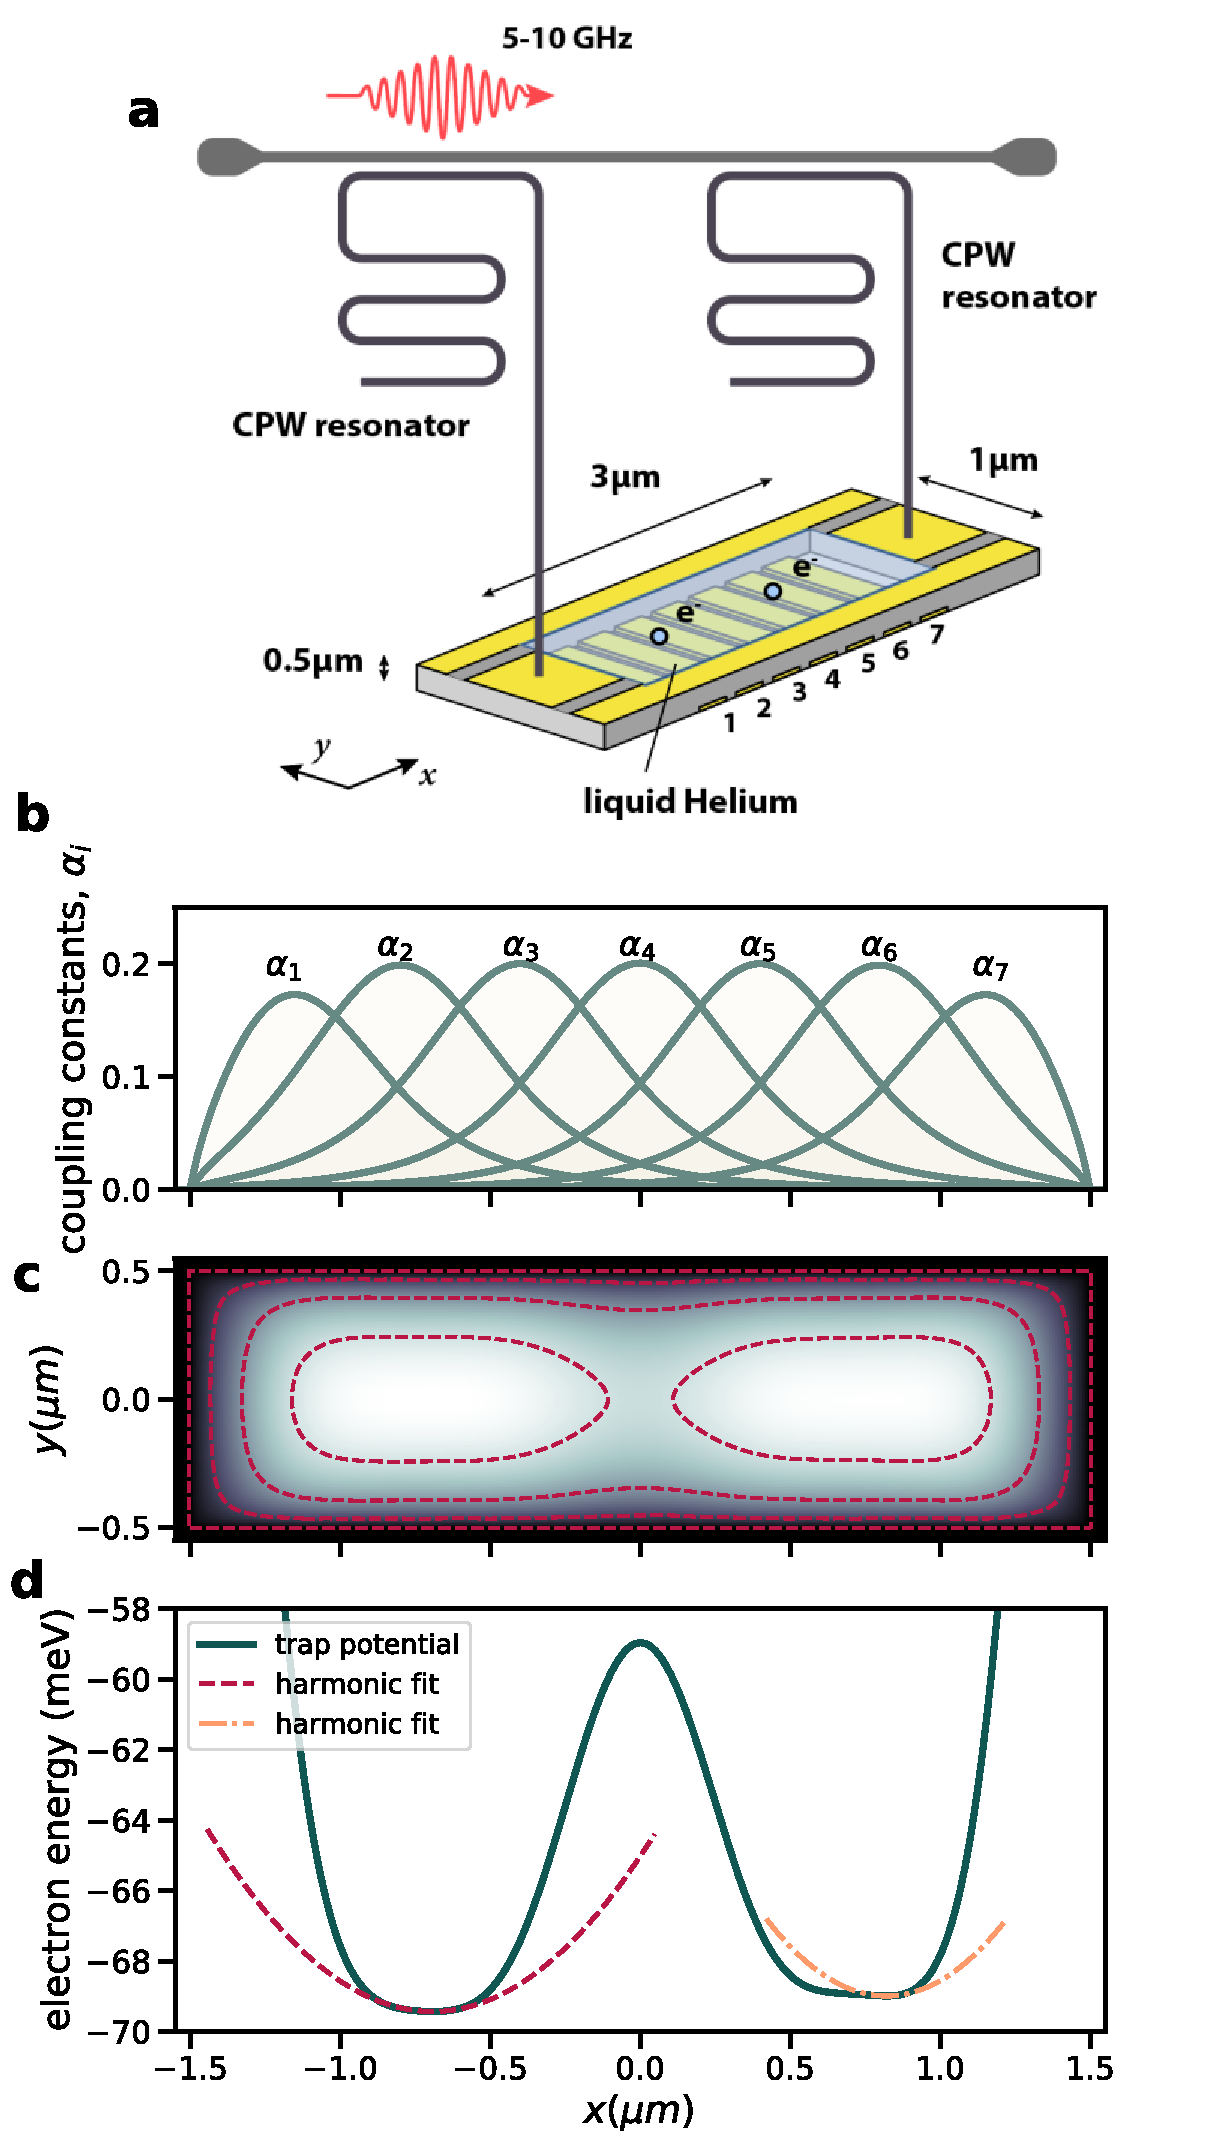
\includegraphics[width=0.49\textwidth]{figure1.pdf}
\caption{\label{fig1} (a) Figure caption. \textcolor{blue}{Niyaz will modify Fig. 1a to include control and readout resonators.}}
\end{figure}

\section{Interaction driven entanglement}

In order to study the importance of level avoided crossings and
entanglement, we study first a simple two-level system. Thereafter we
extend our level-crossing model to a four-level system which can be
interpreted as composed of two separate (not necessarily identical)
subsystems.

We let our Hamiltonian depend linearly on a strength parameter $z$
\[
       H=H_0+\lambda H_\mathrm{I},
\]

with $\lambda \in [0,1]$, where the limits $\lambda=0$ and $\lambda=1$
represent the non-interacting (or unperturbed) and fully interacting
system, respectively.  The model is an eigenvalue problem with only
two available states, which we label $\vert 0\rangle$ and $\vert
1\rangle$, respectively. Below we will let state $\vert 0 \rangle$
represent the lowest state (often referred to as model-space state)
eigenvalue whereas state $\vert 1\rangle$ represents the eigenvalue of
the excluded space.  The non-interacting solutions to our problem are

\[
       H_0\vert 0 \rangle =\epsilon_0\vert 0 \rangle,
\]
and
\[
       H_0\vert 1\rangle =\epsilon_1\vert 1\rangle,
\]

with $\epsilon_0 < \epsilon_1$. We label the off-diagonal matrix
elements $X$, while $X_0=\langle 0 \vert H_I\vert 0 \rangle$ and
$X_1=\langle 1 \vert H_1\vert 1 \rangle$.  The Hamiltonian matrix to be diagonalized is then given by
\[
\left(\begin{array}{cc}\epsilon_0+\lambda X_0 &\lambda X \\
\lambda X &\epsilon_1+\lambda X_1 \end{array}\right).
\]

In the results below we set the parameters $\epsilon_0=0$,
$\epsilon_1=4$, $X_0=-X_1=3$ and $X=0.2$.  This eigenvalue problem can
easily be rewritten in terms of the standard Pauli matrices.  The
non-interacting solutions represent our computational basis.
Pertinent to our choice of parameters, is that at $\lambda\geq 2/3$,
the lowest eigenstate is dominated by $\vert 1\rangle$ while the upper
is $\vert 0 \rangle$. At $\lambda=1$ the $\vert 0 \rangle$ mixing of
the lowest eigenvalue is $1\%$ while for $\lambda\leq 2/3$ we have a
$\vert 0 \rangle$ component of more than $90\%$.  The character of the
eigenvectors has therefore been interchanged when passing $z=2/3$. The
value of the parameter $X$ represents the strength of the coupling
between the model space and the excluded space.  
% add figure here

This  model exhibits a simple level crossing where the
composition of the final interacting states change character as we
gradually switch on the interaction.  In order to study how
entanglement relates to level crossing and the main results of our
investigations, we extend the simple two-level system to a four level
system. This system can be thought of as composed of two subsystems
$A$ and $B$. Each subsystem has computational basis states

\[
\vert 0\rangle_{\mathrm{A,B}}=\begin{bmatrix} 1 & 0\end{bmatrix}^T \hspace{1cm} \vert 1\rangle_{\mathrm{A,B}}=\begin{bmatrix} 0 & 1\end{bmatrix}^T.
\]

The subsystems could represent single particles or composite many-particle systems of a given symmetry.
This leads to the many-body computational basis states
\[
\vert 00\rangle = \vert 0\rangle_{\mathrm{A}}\otimes \vert 0\rangle_{\mathrm{B}}=\begin{bmatrix} 1 & 0 & 0 &0\end{bmatrix}^T,
\]
and
\[
\vert 10\rangle = \vert 1\rangle_{\mathrm{A}}\otimes \vert 0\rangle_{\mathrm{B}}=\begin{bmatrix} 0 & 1 & 0 &0\end{bmatrix}^T,
\]
and
\[
\vert 01\rangle = \vert 0\rangle_{\mathrm{A}}\otimes \vert 1\rangle_{\mathrm{B}}=\begin{bmatrix} 0 & 0 & 1 &0\end{bmatrix}^T,
\]
and finally
\[
\vert 11\rangle = \vert 1\rangle_{\mathrm{A}}\otimes \vert 1\rangle_{\mathrm{B}}=\begin{bmatrix} 0 & 0 & 0 &1\end{bmatrix}^T.
\]
These computational basis states define also the eigenstates of the non-interacting  Hamiltonian
\[
H_0\vert 00 \rangle = \epsilon_{00}\vert 00 \rangle,
\]
\[
H_0\vert 10 \rangle = \epsilon_{10}\vert 10 \rangle,
\]
\[
H_0\vert 01 \rangle = \epsilon_{01}\vert 01 \rangle,
\]
and
\[
H_0\vert 11 \rangle = \epsilon_{11}\vert 11 \rangle.
\]
The interacting part of the Hamiltonian $H_{\mathrm{I}}$ is given by the tensor product of two $\sigma_x$ and $\sigma_z$  matrices, respectively, that is
\[
H_{\mathrm{I}}=H_x\sigma_x\otimes\sigma_x+H_z\sigma_z\otimes\sigma_z,
\]

where $H_x$ and $H_z$ are interaction strength parameters. Our final Hamiltonian matrix is given by
\[
\bm{H}=\begin{bmatrix} \epsilon_{00}+H_z & 0 & 0 & H_x \\
                       0  & \epsilon_{10}-H_z & H_x & 0 \\
                       0 & H_x & \epsilon_{01}+H_z & 0 \\
                       H_x & 0 & 0 & \epsilon_{11} -H_z \end{bmatrix}.
\]

The four eigenstates of the above Hamiltonian matrix can in turn be used to
define density matrices. As an example, the density matrix of the
first eigenstate (lowest energy $E_0$) $\Psi_0$ is

\[
\rho_0=\left(\alpha_{00}\vert 00 \rangle\langle 00\vert+\alpha_{10}\vert 10 \rangle\langle 10\vert+\alpha_{01}\vert 01 \rangle\langle 01\vert+\alpha_{11}\vert 11\
 \rangle\langle 11\vert\right),
\]
where the coefficients $\alpha_{ij}$ are the eigenvector coefficients
resulting from the solution of the above eigenvalue problem.  We can
then in turn define the density matrix for the subsets $A$ or $B$ as

\[
\rho_A=\mathrm{Tr}_B(\rho_{0})=\langle 0 \vert \rho_{0} \vert 0\rangle_{B}+\langle 1 \vert \rho_{0} \vert 1\rangle_{B},
\]
or
\[
\rho_B=\mathrm{Tr}_A(\rho_{\Psi_0})=\langle 0 \vert \rho_{0} \vert 0\rangle_{A}+\langle 1 \vert \rho_{0} \vert 1\rangle_{A}.
\]

The density matrices for these subsets can be used to compute the
so-called von Neumann entropy, which is one of the possible measures
of entanglement. A pure state has entropy equal zero while entangled
state have an entropy larger than zero. The von Neumann entropy is
defined as
\[
S(A,B)=-\mathrm{Tr}\left(\rho_{A,B}\log_2 (\rho_{A,B})\right).
\]
The example here shows the above von Neumann entropy based on the
density matrix for the lowest many-body state. We see clearly a jump
in the entropy around the point where we have a level crossing. At
interaction strength $\lambda=0$ we have many-body states purely
defined by their computational basis states. As we switch on the
interaction strength, we obtain an increased degree of mixing and the
entropy increases till we reach the level crossing point where we see
an additional and sudden increase in entropy. Similar behaviors are
observed for the other states. The most important result from this
example is that entanglement is driven by the Hamiltonian itself and
the strength of the interaction matrix elements and the
non-interacting energies.

% add figs here

With these introductory examples, we are now in the position where we
can start to interpret and model realistic interacting many-electron
systems in terms of the strength of the Coulomb interaction and the
shapes of the potential well. Our specific system is composed of two
potential wells with one fermion (electrons in our case) trapped in
each well.  Each potential well can sustain a certain number of bound
single-particle states and defines our subsystems $A$ and $B$. The
non-interacting part of the Hamiltonian is given by the mere addition
of the single-particle energies from each repsective well (make figure
with labels A and B and single-particle energies).

The eigenstates of the non-interacting Hamiltonian $H_0$ are given by
various computational basis states with the difference from the above
simple models that now we have more than two states in each
subsystem. The depths of the potential wells and their respective
distances can be tuned in an experimental set up. The theoretical
calculations presented here can thus serve as a tool which aids in
finding the optimal parameters in order to study entanglement in a
many-body environment.

What follows is a description of the theoretical models used to
simulate the two-electron system. 

\section{Entanglement in quantum dot systems} % Hakon, Oyvind
    As we are studying a model comprised of two electrons restricted to move in a
    one-dimensional external potential we have employed exact diagonalization of the
    two-body Schrödinger equation to solve the problem.
    We build a two-particle wave function from a set of single-particle
    functions.
    The basis of single-particle functions we will use are eigenstates of the
    one-body Hamiltonian represented on a discrete grid.
    This allows for flexibility in the choice of the external potential, and fits the
    interpolated potential particularly well.

    \subsection{The Hamiltonian}
        The full Hamiltonian for two interacting electrons in an external
        potential $v(x)$ is given by
        \begin{align*}
            \hat{H}
            = \sum_{i = 1}^{2}\qty(
                -\frac{\hbar^2}{2m}\dv[2]{}{x_i}
                + v(x_i)
            )
            + u(x_1, x_2),
        \end{align*}
        where we use a soft-Coulomb interaction $u(x_1, x_2)$ given by
        \begin{align}
            u(x_1, x_2)
            =
            \frac{\alpha}{\sqrt{\qty(x_1 - x_2)^2 + a^2}},
            \label{eq:soft-coulomb}
        \end{align}
        where we have set $e = (4 \pi \epsilon_0)^{-1} = 1$.
        % Note: Scaling should maybe be discussed in full when introducing kappa
        Here $\alpha$ adjusts the strength of the interaction, and $a$ removes
        the singularity at $x_1 = x_2$.
        The Coulomb interaction is symmetric with respect to the positions and
        $u(x_1, x_2) = u(x_2, x_1)$.
        The kinetic energy operator and the external potential $v(x_i)$ constitutes
        the one-body part of the Hamiltonian.
        We will denote the one-body Hamiltonian by $\hat{h}$.
        There is no spin-dependence in this system, and we will restrict our attention
        to the spatial part of the problem.
        % TODO: Reference work discussing the suitability of this for the liquid
        % helium system.
        % This can be done by referring to the section on spin considerations.
        For numerical analysis we wish to use a dimensionless expression for the
        Hamiltonian.
        This is done by...
        % Note: Recap the steps needed to construct the dimensionless Hamiltonian.
        % TODO: Niyaz will handle this in the introduction

    \subsection{Constructing the single-particle basis sets}
        As much of the analysis will be performed by varying the shape and
        strength of the interpolated external potential we deem a flexible
        finite-difference basis set a suitable candidate.
        % TODO: List some other alternatives such as e.g., gaussians and DVR.
        The single-particle time-independent one-dimensional system can be
        described by the one-body Hamiltonian
        \begin{align*}
            h(x) = -\frac{1}{2}\dv[2]{}{x}
            + v(x),
        \end{align*}
        where the external potential $v(x)$ is an arbitrary function of the grid $x$.
        We proceed by discretizing the grid into $N_g$ uniform points with a spacing
        $\Delta x$ and use the second-order central differences method for the
        double-derivative.
        Building a tridiagonal matrix from the grid points, we solve the eigenvalue
        equation and choose the $l \leq N_g$ first eigenstates (i.e., the eigenstates
        with the lowest eigenenergy) as the single-particle basis
        $\{\psi_i\}_{i = 1}^l$.
        These basis states will be normalized with respect to the dot product (as we
        find the coefficients of the discretized grid).
        That is, $\sum_{j = 1}^{N_g} | \psi_i(x_j) |^{2} = 1$, however we want our
        states to be normalized with respect to the integral which entails a
        differential $\dd{x} \approx \Delta x$.
        As our grid is uniform we can then normalize the single-particle states
        by $\psi_i(x_j) \to \psi_i(x_j) / \sqrt{\Delta x}$.
        We then get $\braket{\psi_i}{\psi_j} = \delta_{ij}$ and the one-body matrix
        elements are given by
        \begin{align*}
            h_{ij} \equiv \mel{\psi_i}{\hat{h}}{\psi_j}
            = \delta_{ij}\varepsilon_j,
        \end{align*}
        where $\varepsilon_j$ are the eigenenergies.

        Now, for the specific problem that  we are solving the system is described
        by two deep wells $v^{L}(x)$ and $v^{R}(x)$, where $L$ and $R$ are labels
        for the left and right well respectively.
        The wells will be so deep that there will be no tunneling over the
        barrier in the bound states that we will use for our single-particle
        basis.
        Furthermore, the Coulomb repulsion will be strong enough to ensure that
        we will not see any two-body eigenstates with two particles in one of
        the wells for the energy levels that we are interested in.
        % TODO: We will not see these states for the distinguishable model
        % as we force one particle to be in each well.
        This makes the system split up into two distinguishable subsystems
        that we label $L$ and $R$ with one particle in each subsystem.
        In order to distinguish these systems from one another in the
        two-particle picture we will construct two disjoint single-particle
        basis sets $\qty{\phi^{L}_{i}}_{i = 1}^{N_L}$ and
        $\qty{\phi^{R}_{i}}_{i = 1}^{N_R}$, where
        $\braket{\phi^{A}_{i}}{\phi^{B}_{j}} = \delta^{AB} \delta_{ij}$
        \footnote{
            It is worth pointing out that we will not see any products
            between states in different wells.
            We can in this problem think of the two basis sets as living in
            two different Hilbert spaces as would be done for e.g., the
            Jaynes-Cummings systems where there are no overlap elements
            between the photonic and the electronic states.
        }.
        % TODO: Are the single-particle basis states the computational basis
        % elements?
        Using the finite-difference approach described above we can set up this
        basis in two different ways.
        The first is to diagonalize the full one-body Hamiltonian
        \begin{align*}
            h(x) = -\frac{1}{2} \dv[2]{}{x} + v^{L}(x) + v^{R}(x),
        \end{align*}
        and then sort the eigenstates by which well they are localized in.
        To do this we can compute the center of mass of the single-particle
        wave function and see where it is centered.
        % TODO: Maybe include a plot of this? Optionally in a supplementary
        % materials.
        The drawback when using this method is that we must include a large
        number of basis states when the wells are far detuned.
        This is because the eigenstates with the lowest eigenvalue are best
        described.
        Therefore, to localize states in the highest energy well will require
        very high energy states.
        % TODO: Discuss this fact a little more. It can also be enough to
        % demonstrate that the we need a lot of grid points to construct the
        % eigenstates in one of the wells properly.

        The second approach is to \emph{a priori} determine that the
        eigenstates will split up into two disjoint sets, where
        $v^{L}(x) \phi^{R}(x) = v^{R}(x) \phi^{L}(x) = 0$.
        % TODO: This condition should be tested explicitly.
        % TODO: Add a plot of this.
        We can then construct two one-body Hamiltonian operators given
        by
        \begin{align*}
            h^{A}(x) \equiv -\frac{1}{2} \dv[2]{}{x} + v^{A}(x),
        \end{align*}
        that we can separately diagonalize, and construct a set of
        single-particle eigenpairs for each well.
        For the potential wells we describe both approaches will give the
        same eigenpairs to numerical precision.
        % TODO: This should be backed up, and formulated a little differently.
        % Perhaps included in a supplemental material?
        The two sets of matrix elements for the one-body Hamiltonian will
        then be
        \begin{align*}
            h^{A}_{ij}
            \equiv \mel*{\phi^A_i}{\hat{h}^A}{\phi^A_j}
            = \delta_{ij} \epsilon^{A}_j,
        \end{align*}
        where $\epsilon^A_i$ are the eigenenergies of $\hat{h}^A$.
        We then have that $\braket*{\phi^A_i}{\phi^B_j} = \delta^{AB}
        \delta_{ij}$ as the two sets of basis states are so far removed
        that they share no overlap (hence, $\delta^{AB}$), and as they
        are eigenstates (hence, $\delta_{ij}$).


    \subsection{Describing the two-body problem}
        Due to there only being two particles we will solve the full problem
        using exact diagonalization \footnote{
            By ``exact'' we here mean that the solution is exact within the
            truncated, approximate, finite-difference basis set.
        }, often denoted the \emph{full configuration interaction} method
        in electronic structure theory \cite{the-pink-book}.
        The wave function ansatz is then given by
        \begin{align*}
            \ket*{\Psi_I}
            &= \sum_{k = 1}^{N_L} \sum_{l = 1}^{N_R} C_{kl, I}
            \ket*{\phi^{L}_k \phi^{R}_l},
        \end{align*}
        where no symmetry is assumed for the wave function, and the index
        $I = (i, j)$ is a compound index denoting the excited two-body
        state we are looking at.
        We denote the two-particle product state as $\ket*{\phi^L_i \phi^R_j}
        \equiv \ket*{\phi^L_i} \otimes \ket*{\phi^R_j}$.
        There will be a total of $N_L N_R$ eigenstates $\ket*{\Psi_I}$.
        We adopt the notation $\bra*{\phi^L_i \phi^R_j}
        = \bra*{\phi^L_i} \otimes \bra*{\phi^R_j}
        \equiv \ket*{\phi^L_i \phi^R_j}^{\dagger}$.
        This should be contrasted with the conventional way of doing full
        configuration interaction in electronic structure theory by using
        a linear combination of Slater determinants as the electrons are
        indistinguishable \cite{the-pink-book}.

        For the full many-body system we need the matrix elements of the
        soft-Coulomb interaction operator $u(x_1, x_2)$ from
        equation \eqref{eq:soft-coulomb}.
        As we are using a finite-difference basis set, we will compute the matrix
        elements using numerical integration.
        That is, we compute the matrix elements
        \begin{align}
            u_{ij, kl}
            &\equiv \mel*{\phi^L_i\phi^R_j}{\hat{u}}{\phi^L_k\phi^R_l}
            \\
            &= \int\dd{x_1} \dd{x_2}
            {\phi^L_i}^{*}(x_1) {\phi^R_j}^{*}(x_2)
            \nonumber \\
            &\qquad
            \times
            u(x_1, x_2)
            \phi^L_k(x_1)\phi^R_l(x_2),
            \label{eq:two-body-coulomb}
        \end{align}
        by the use of the trapezoidal rule integrating over $x_2$ first.
        This entails to constructing the matrix elements $W_{ij}(x)$
        given by
        \begin{align*}
            W_{ij}(x)
            = \int \dd{y} {\phi^R_i}^{*}(y) u(x, y) \phi^R_j(y),
        \end{align*}
        and use this to compute the two-body matrix elements from
        \begin{align*}
            u_{ij, kl}
            = \int \dd{x_1} {\phi^{L}_{i}}^{*}(x_1)
            W_{jl}(x_1) \phi^L_k(x_1),
        \end{align*}
        where we note in passing that all the single-particle eigenstates
        are real.
        Furthermore, the choice of constructing $W_{ij}(x)$ by integrating
        first over $x_2$, i.e., the right well, is completely arbitrary.
        Integrating over the left well first, and then the right well gives
        exactly the same matrix elements $u_{ij, kl}$ due to the symmetry
        of the Coulomb interaction.

        Inserting the wave function ansatz into the time-independent Schrödinger
        equation, and projecting onto a two-body state
        $\bra*{\phi^L_i \phi^R_j}$ we get
        \begin{align*}
            \mel*{\phi^L_i \phi^R_j}{\hat{H}}{\Psi_K}
             % &= \sum_{k = 1}^{N_L} \sum_{l = 1}^{N_R}
             % \mel*{\phi^L_i \phi^R_j}{\hat{H}}{\phi^L_k \phi^R_l}
             % C_{kl, K}
             % \\
            &= \sum_{k = 1}^{N_L} \sum_{l = 1}^{N_R}
            H_{ij, kl} C_{kl, K}
            = S_{ij, kl} C_{kl, K} E_{K},
        \end{align*}
        where $H_{ij, kl} \equiv \mel*{\phi^L_i \phi^R_j}{\hat{H}}{
        \phi^L_k \phi^R_l}$ are the matrix elements of the Hamiltonian in
        the product basis, and $S_{ij, kl} = \braket*{
        \phi^L_i \phi^R_j}{\phi^L_k \phi^R_l} = \delta_{ik} \delta_{jl}$ are
        the overlap matrix elements between two two-body states.
        Solving this generalized eigenvalue equation gives us the
        coefficients $C_{ij, K}$ where the columns correspond to the
        eigenstates $\ket*{\Psi_K}$, and the eigenenergies $E_K$.
        As discussed in the previous section we know that the one-body Hamiltonian
        will split up into two disjoint operators; one for the left-well and the
        other for the right-well.
        We can write the one-body Hamiltonian as $\hat{h} = \hat{h}^L \otimes \hat{1}
        + \hat{1} \otimes \hat{h}^{R}$.
        From the orthonormality of the two sets of eigenstates we get
        \begin{align}
            h_{ij, kl}
            &= \mel*{\phi^L_i \phi^R_j}{\hat{h}}{\phi^L_k \phi^R_l}
            % \\
            % &= \mel*{\phi^{L}_i}{\hat{h}^L}{\phi^L_k}
            % \braket*{\phi^R_j}{\phi^R_l}
            % + \braket*{\phi^L_i}{\phi^L_k}
            % \mel*{\phi^R_j}{\hat{h}^R}{\phi^{R}_l}
            % \\
            % &=
            % \delta_{ik} \epsilon^{L}_k
            % \delta_{jl}
            % + \delta_{ik}
            % \delta_{jl} \epsilon^{R}_l
            = \delta_{ik} \delta_{jl} \qty(
                \epsilon^L_k
                + \epsilon^{R}_l
            ).
            \label{eq:one-body-hamiltonian}
        \end{align}
        From the matrix elements of the one-body Hamiltonian in
        \eqref{eq:one-body-hamiltonian} and the Coulomb operator
        \eqref{eq:two-body-coulomb} we can construct the full Hamiltonian
        to be $H_{ij, kl} = h_{ij, kl} + u_{ij, kl}$.
        We then proceed to diagonalize the matrix, and find the coefficients
        $C_{kl, K}$ and the corresponding eigenenergies $E_K$.

    \subsection{Spin considerations}
        We have so far in this discussion ignored the spin component of the electrons.
        As we are considering two electrons we expect to see singlet and triplet
        configurations for the total wave function.
        The Hamiltonian is spin-independent and we can therefore limit our attention
        to the spatial components of the wave functions.
        % TODO: Add reference to the lack of spin interactions in the liquid helium
        % system?
        Furthermore, as the system is described by a double-well with a separate
        spatial basis for each well, we know that the singlet and the triplet states
        will be degenerate for all states where there is one particle in each well
        (which is the only case we consider in this work),
        and we can fully factorize out the spin-part of the problem.


    \subsection{Measuring the degree of entanglement}
        % TODO: Why do we need entanglement?
        % Add reference to the quantum computing books.
        As we have diagonalized the Hamiltonian and found the energy spectrum, we
        in principle have all the knowledge that can be obtained from the system.
        We also work in a zero-temperature regime with no noise from the outside
        world.
        This lets us create a pure state from the two-particle wave function.
        % TODO: Which states are we interested in measuring entanglement for?

        For a given two-body pure state $\ket*{\Psi}$ we can construct the
        corresponding density operator
        \begin{align*}
            \hat{\rho} = \dyad*{\Psi}{\Psi}
            = C_{ij} C^{*}_{kl} \dyad*{\phi^L_i \phi^R_j}{
                \phi^L_k \phi^R_l
            },
        \end{align*}
        where $C_{ij}$ are the coefficients \footnote{
            Note that these coefficients are not necessarily the eigenstates
            of the full two-body Hamiltonian.
            We are free to choose whatever state we wish as long as the states
            are normalized.
        }.
        A measure of entanglement can be achieved from the von Neumann entropy.
        We then need to construct the reduced density operators for each
        subsystem $L$ and $R$.
        They are given by
        \begin{gather*}
            \hat{\rho}^L
            = \tr_R \! \qty(\hat{\rho})
            = C_{ij} C^{*}_{kj} \dyad*{\phi^L_i}{\phi^L_k},
            \\
            \hat{\rho}^R
            = \tr_{L} \! \qty(\hat{\rho})
            = C_{ij} C^{*}_{il} \dyad*{\phi^R_j}{\phi^R_l},
        \end{gather*}
        where we have used that the single-particle states in each well are
        orthonormal.
        As the total state is a pure state, we know that the reduced density
        operators must have the same spectrum (the von Neumann entropies must
        cancel perfectly).
        In the case where there are indistinguishable particles the one-body
        density can be used as a replacement for the reduced density matrices
        of the two subsystems.
        We can construct the one-body density operator from $\hat{\rho}^1
        = \hat{\rho}^L + \hat{\rho}^R$.
        % TODO: Describe how measurement is performed using the reduced density
        % operators.
        % We can compute the expectation value of the energy in the subsystems.
        % TODO: Describe the avoided crossing

 

        
% TODO: Plot the coefficients of the eigenstates in well
% configuration far from the avoided crossing, and close
% to the avoided crossing.
\begin{figure}
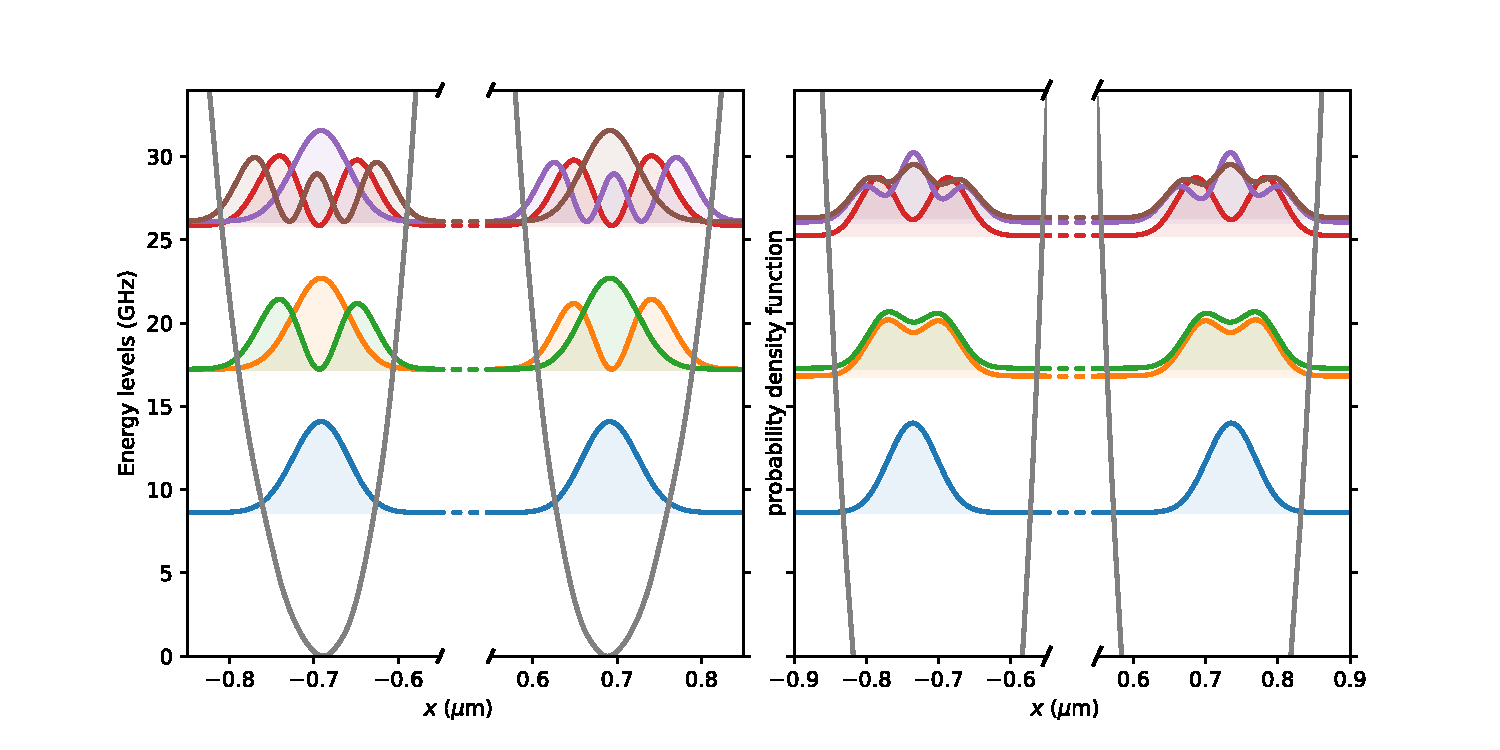
\includegraphics[width=0.49\textwidth]{figure2.pdf}
\caption{\label{fig2} (a) Figure caption.}
\end{figure}

\section{Results and Discussion} % all of us

\begin{figure}
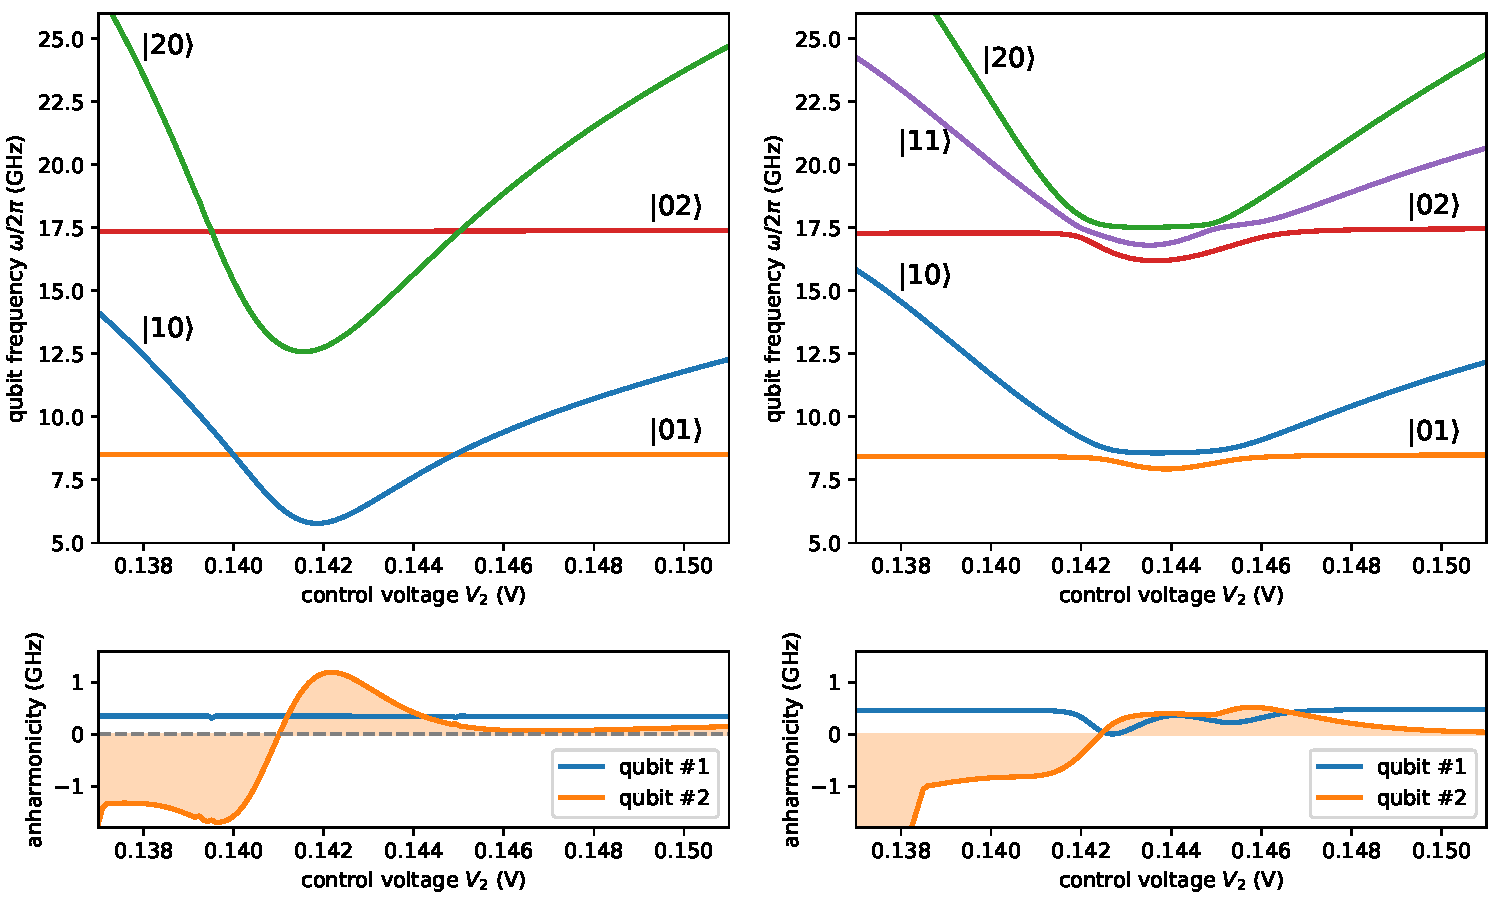
\includegraphics[width=0.49\textwidth]{figure3.pdf}
\caption{\label{fig3} (a) Figure caption.}
\end{figure}

% TODO: Plot the entropy as a function of the well
% configurations.

\section{Conclusions} % we can wait to write this one until the end

\section{\label{sec:level1}Problem: Many-level system interacting with EM field}

We start with the following problem in general form: we have a quantum-mechanical system described with Hamiltonian $H_0$ and states $\ket{n}$ being eigenfunctions of $H_0$.
\begin{equation*}
H_0 \ket{n} = E_n \ket{n}
\end{equation*}
We would like to know how these states evolve in time in the presence of a time-varying electric field. The interaction of quantum systems with electric fields is described by the Hamiltonian $ H_i = - \vb{E}(t) \vb{d}$, where $\vb{E}(t) = \vb{\mathcal{E}}_0 \cos \omega t$ and $\vb{d}$ is the dipole moment of the quantum system. Note, here we use dipole approximation (wavelength of the EM field is much larger than characteristic size of the quantum system wavefunction). The evolution of the quantum wavefunction is governed by Schrodinger equation:
\begin{equation}
 i \dot{\psi} = H \psi
\label{eq1}.
\end{equation}
where $H = H_0 + H_i$ (note, $\hbar = 1$). We seek the solution in the form $\psi(t) = \sum_n C_n(t) e^{-i E_n t}$. We evolve this solution through Eq.~\ref{eq1} and get the following answer:
\begin{equation}
 i \dot{C_m} = -\frac{1}{2} \vb{\mathcal{E}}_0 \sum_{\alpha} \sum_{n} C_n e^{i \omega_{mn} t + i \alpha \omega t} \vb{d}_{mn}
\label{eq2},
\end{equation}
\begin{equation}
 \braket{m}{n} = \delta_{mn}, \mel{m}{\vb{d}}{n} = \vb{d}_{mn}, E_m - E_n = \omega_{mn}
\end{equation}
Here we used $\cos \omega t = \frac{1}{2} \sum_{\alpha = \pm} e^{i \alpha \omega t}$. Lets assume the system is in the ground state at $t = 0$, so $C_n(0) = \delta_{n1}$. We integrate Eq.~\ref{eq2} and get an expression:
\begin{equation}
 C_m = \frac{i}{2} \vb{\mathcal{E}}_0 \sum_{\alpha} \vb{d}_{m1} \frac{e^{i (\omega_{mn} + \alpha \omega) t} - 1}{i (\omega_{m1} + \alpha \omega)} 
\label{eq3}.
\end{equation}
An important condition here is:
\begin{equation}
\abs{\frac{\vb{\mathcal{E}}_0 \vb{d}_{m1}}{\omega_{m1} \pm \omega}} \ll 1
\label{eq4},
\end{equation}
which defines the 2-level approximation

\section{Appendix A}
Description of classical two-body calculation


\begin{acknowledgments}
We are grateful to M.I. Dykman and S.A. Lyon for illuminating discussions. The work of MHJ is supported by the U.S. Department of Energy, Office of Science, office of Nuclear Physics under grant No. DE-SC0021152 and U.S. National Science Foundation Grants No. PHY-1404159 and PHY-2013047. JP acknowledges support from the National Science Foundation via grant number DMR-2003815 as well as the valuable support of the Cowen Family Endowment at MSU. The work of NRB is supported by a sponsored research grant from EeroQ Corp. JP and NRB thank J.R. Lane and J.M. Kitzman for illuminating discussions.
\end{acknowledgments}
\bibliography{apssamp}% Produces the bibliography via BibTeX.

\end{document}
%
% ****** End of file apssamp.tex ******
